\section{Step-by-Step Linearizability of Extended Priority Queues}
\label{sec:step-by-step linearizability of extended priority queues}

In this section we shows that, with the help of a property called step-by-step linearizability, we can partition the concurrent executions which are not linearizable with respect to $\textit{EPQ}$ into a finite number of classes. Intuitively, each such class represents a set of sequential execution that violate one rule of extended priority queue. Here step-by-step linearizability enables us to build a linearization for an execution $e$ incrementally, using linearizations of projections of $e$. Our step-by-step linearizability is inspired by the step-by-step linearizabilility of queue and stacks in \cite{Bouajjani:2015}. The proof of lemmas in this section can be found in Appendix \ref{sec:appendix in section step-by-step linearizability of extended priority queues}.

The projection $e \vert{\mathcal{D}}$ of a sequential execution $e$ into a subset $\mathcal{D} \subseteq \mathbb{D}$ of items is obtained from $e$ by erasing all method events with a data value not in $\mathcal{D}$. The set of projections of $e$ is denoted $\textit{proj}(e)$. When refer to $\textit{proj}(e)$, we implicitly assume that each $\textit{rm}(\textit{empty})$ in $e$ has a ghost argument that is unique. We write $e \setminus x$ for the projection $e \vert_{ \mathbb{D} \setminus \{ x \} }$. This extends naturally to histories and concurrent executions.

A set $S$ of sequential executions is closed under projection, if for all $\mathcal{D} \subseteq \mathbb{D}$ and $e \in S$, we have $e \vert_{ \mathcal{D} } \in S$. The following lemma states that $\textit{EPQ}$ is closed under projection, since the predicates used in rules of extended priority queue are ``closed under projection''.

\begin{restatable}{lemma}{EPQisClosedUnderProjection}
\label{lemma:EPQ is closed under projection}
$\textit{EPQ}$ is closed under projection.
\end{restatable}

A sequential execution $e$ matches a rule $R$ of extended priority queue, if $e=\textit{Expr}(l_1, \ldots, l_k,a,b)$, and $\textit{Guard}(l_1, \ldots, l_k,a,b)$ holds. Here $\textit{Guard}$ and $\textit{Expr}$ are of rule $R$, and we call $a$ (if exists) the witness of $e$. We denote by $\textit{MS}(R)$ the set of sequential executions which match $R$. Note that sequences in $\textit{MS}(R)$ only respect rule $R$ and may be not in $\textit{EPQ}$. $e$ is linearizable with respect to $\textit{MS}(R)$ with witness $x$, if $e$ is linearizable with respect to $u \in \textit{MS}(R)$ and $x$ is the witness of $u$.

\begin{example}\label{example:match set of R}
Assume that $p_1 <_{\mathbb{P}} p_2$, we can see that $e = \textit{rm}(b) \cdot \textit{put}(b,p_1) \cdot \textit{put}(a,p_2) \cdot \textit{rm}(a)$ is in $\textit{MS}(\textit{EPQ}_1^{>} )$, but it is obvious that $e \notin \textit{EPQ}$.
\end{example}

The following lemma states that for data-differentiated sequential execution, checking inclusion into $\textit{EPQ}$ is equivalent to checking inclusion into $\textit{MS}(R)$ for everyone of its projections.

\begin{restatable}{lemma}{EPQasMultiInMRpriforSequence}
\label{lemma:EPQ as multi in MRpri for sequence}
Given a data-differentiated sequential execution $e$, $e \in \textit{EPQ}$, if and only if, $\forall e' \in \textit{proj}(e)$ and $\forall R \in \textit{last}(e')$, we have $e' \in \textit{MS}(R)$.
\end{restatable}

Lemma \ref{lemma:EPQ as multi in MRpri for sequence} simplifies checking inclusion into $\textit{EPQ}$, since checking $\textit{MS}(R)$ only concerns information of one rule, while checking $\textit{EPQ}$ need to consider every method events. We want a similar lemma for checking linearizability with respect to $\textit{EPQ}$. To enable such equivalent characterization, we introduce the notion of step-by-step linearizability for extended priority queue. The projection $e \vert{O}$ of a concurrent execution $e$ into a set $O$ of operations is obtained from $e$ by erasing all call and return actions of non-$O$ operations. We write $e \setminus o$ for the projection $e \vert_{ O_h \setminus \{ o \} }$, where $O_h$ is the set of operations of $e$. This extends naturally to histories. Similarly we can define projection into method events.

\begin{definition}\label{def:step-by-step linearizability of extended priority queue}
A set $S$ of sequential executions of extended priority queue is step-by-step linearizable, if for any data-differentiated execution $e$,
\begin{itemize}
\setlength{\itemsep}{0.5pt}
\item[-] if $e$ is linearizable w.r.t. $\textit{MS}(R)$ ($R \in \{ \textit{EPQ}_1^{>}, \textit{EPQ}_1^{=}, \textit{EPQ}_2^{>},\textit{EPQ}_2^{=} \}$) with witness $x$, we have: $e \setminus x \sqsubseteq \textit{EPQ} \Rightarrow e \sqsubseteq \textit{EPQ}$.

\item[-] if $e$ is linearizable w.r.t. $\textit{MS}(\textit{EPQ}_3)$ and $o$ is a $\textit{rm}(\textit{empty})$ event, we have:

$e \setminus o \sqsubseteq \textit{EPQ} \Rightarrow e \sqsubseteq \textit{EPQ}$.
\end{itemize}
\end{definition}

Given a data-differentiated execution and its history, we can abuse notation and mix labels and method events with operations themselves, since items are unique in a data-differentiated execution. For instance, we will reference an operation labeled by $\textit{put}(p,a)$ as $\textit{put}(p,a)$. The following lemma states that $\textit{EPQ}$ is step-by-step linearizability.

\begin{restatable}{lemma}{EPQueueisStepByStepLinearizability}
\label{lemma:EPQ is step-by-step linearizability}
$\textit{EPQ}$ is step-by-step linearizability.
\end{restatable}

Let us briefly explain the idea of proving step-by-step linearizability of $\textit{EPQ}_1$ with an example, while the other two rules is much simpler to deal with. Given a data-differentiated concurrent execution $e \sqsubseteq l \in \textit{MS}(\textit{EPQ}_1)$ with witness $x$ and assume that $e \setminus x \sqsubseteq l' \in \textit{EPQ}$, we explicitly construct a sequence $l''$ and prove that $e \sqsubseteq l'' \in \textit{EPQ}$. The construction of $l''$ is as follows:

\begin{itemize}
\setlength{\itemsep}{0.5pt}
\item[-] In \figurename~\ref{fig:concurrent execution for EPQ1}, we give an example of $e$, and we explicitly draw the linearization points according to $l'$. Assume that $p_1 <_{\mathbb{P}} p_2$ and $p_1 <_{\mathbb{P}} p_3$. According to $\textit{EPQ}_1$, there exists $u$, $v$ and $w$, such that $l = u \cdot \textit{put}(x,\textit{pri}_x) \cdot v \cdot \textit{rm}(x) \cdot w$. We use $\textit{put}(z_2,p_3)-w$ to denote that $\textit{put}(z_2,p_3)$ is in $w$.

\item[-] Let $O_c$ and $O_i$ be the set of operations with priorities comparable with $\textit{pri}_x$ and incomparable with $\textit{pri}_x$ in $l$, respectively. It seems that we can make $l''= l''_1 \cdot \textit{put}(x,\textit{pri}_x) \cdot l''_2 \cdot \textit{rm}(x) \cdot l''_3$, where $l''_1$, $l''_2$ and $l''_3$ are sequences of operations chosen from $u$, $v$ and $w$, respectively. However, this is incorrect. The reason is that there is no restriction to $O_i$ operations in $u \cdot v$, and thus, there is no guarantee that the projection of $l'$ into $O_i$ operations in $u \cdot v$ being correct. In our example, we can see that such projection is $\textit{put}(z_1,p_3) \cdot \textit{rm}(z_2)$ and is incorrect.

\item[-] Let $U$, $V$ and $W$ be the set of operations in $u$, $v$ and $w$, respectively. We use a two-steps method to construct $U'$, $V'$ and $W'$, which are the new version of $U$, $V$ and $W$.

\item[-] The first step is to obtain $U' \cup V'$ and $W'$. We leave $O_c$ operations unchanged for $U \cdot V$ and $W$. We try to put as many as possible $O_i$ operations into $U' \cup V'$ (regardless whether they belong to $U \cdot V$ or $W$), until we meet a $O_i$ operation $o$ that happens before a $O_c$ operation in $W$. We move $O_i$ operations that before $o$ in $l'$ into $U' \cdot V'$, and move $o$ and $O_i$ operations that after $o$ in $l'$ into $W'$. In this example, $o$ is $\textit{put}(x_3,p_2)$ (emphasized by adding vertical dashed line), we move $\textit{put}(z_1,p_3)$ and $\textit{put}(z_2,p_3)$ into $U' \cdot V'$, and move $\textit{rm}(z_1)$ and $\textit{rm}(z_2)$ into $W'$ (emphasized by adding boxes).

\item[-] The second step is to obtain $U'$ and $V'$. $U'$ contains the following two kinds of operations: (1) Operations whose linearization points are before $\textit{ret}(\textit{put},x)$, and (2) other $\textit{put}$ operations with priority $\textit{pri}_x$. $V'$ contains the remanning operations. In this example, $U'$ contains $\textit{put}(z_1,p_3)$ and $\textit{put}(x_2,p_2)$.

\item[-] $l''_1$ is the concatenation of projection of $l'$ into the first and second kinds of operations in $U'$. $l''_2$ and $l''_3$ are projection of $l'$ into $V'$ and $W'$, respectively. In this example, $l''_1 = \textit{put}(z_1,p_3) \cdot \textit{put}(x_2,p_2)$, $l''_2 = \textit{put}(z_2,p_3) \cdot \textit{rm}(x_2) \cdot \textit{put}(y_1,p_1) \cdot \textit{rm}(y_1)$, and $l''_3 = \textit{put}(x_3,p_2) \cdot \textit{rm}(z_1) \cdot \textit{rm}(z_2)$. In \figurename~\ref{fig:concurrent execution with new linearization points for EPQ1}, we add linarization points according to $l''$, and we can see that $l''$ holds as required.
\end{itemize}

\begin{figure}[htbp]
  \centering
  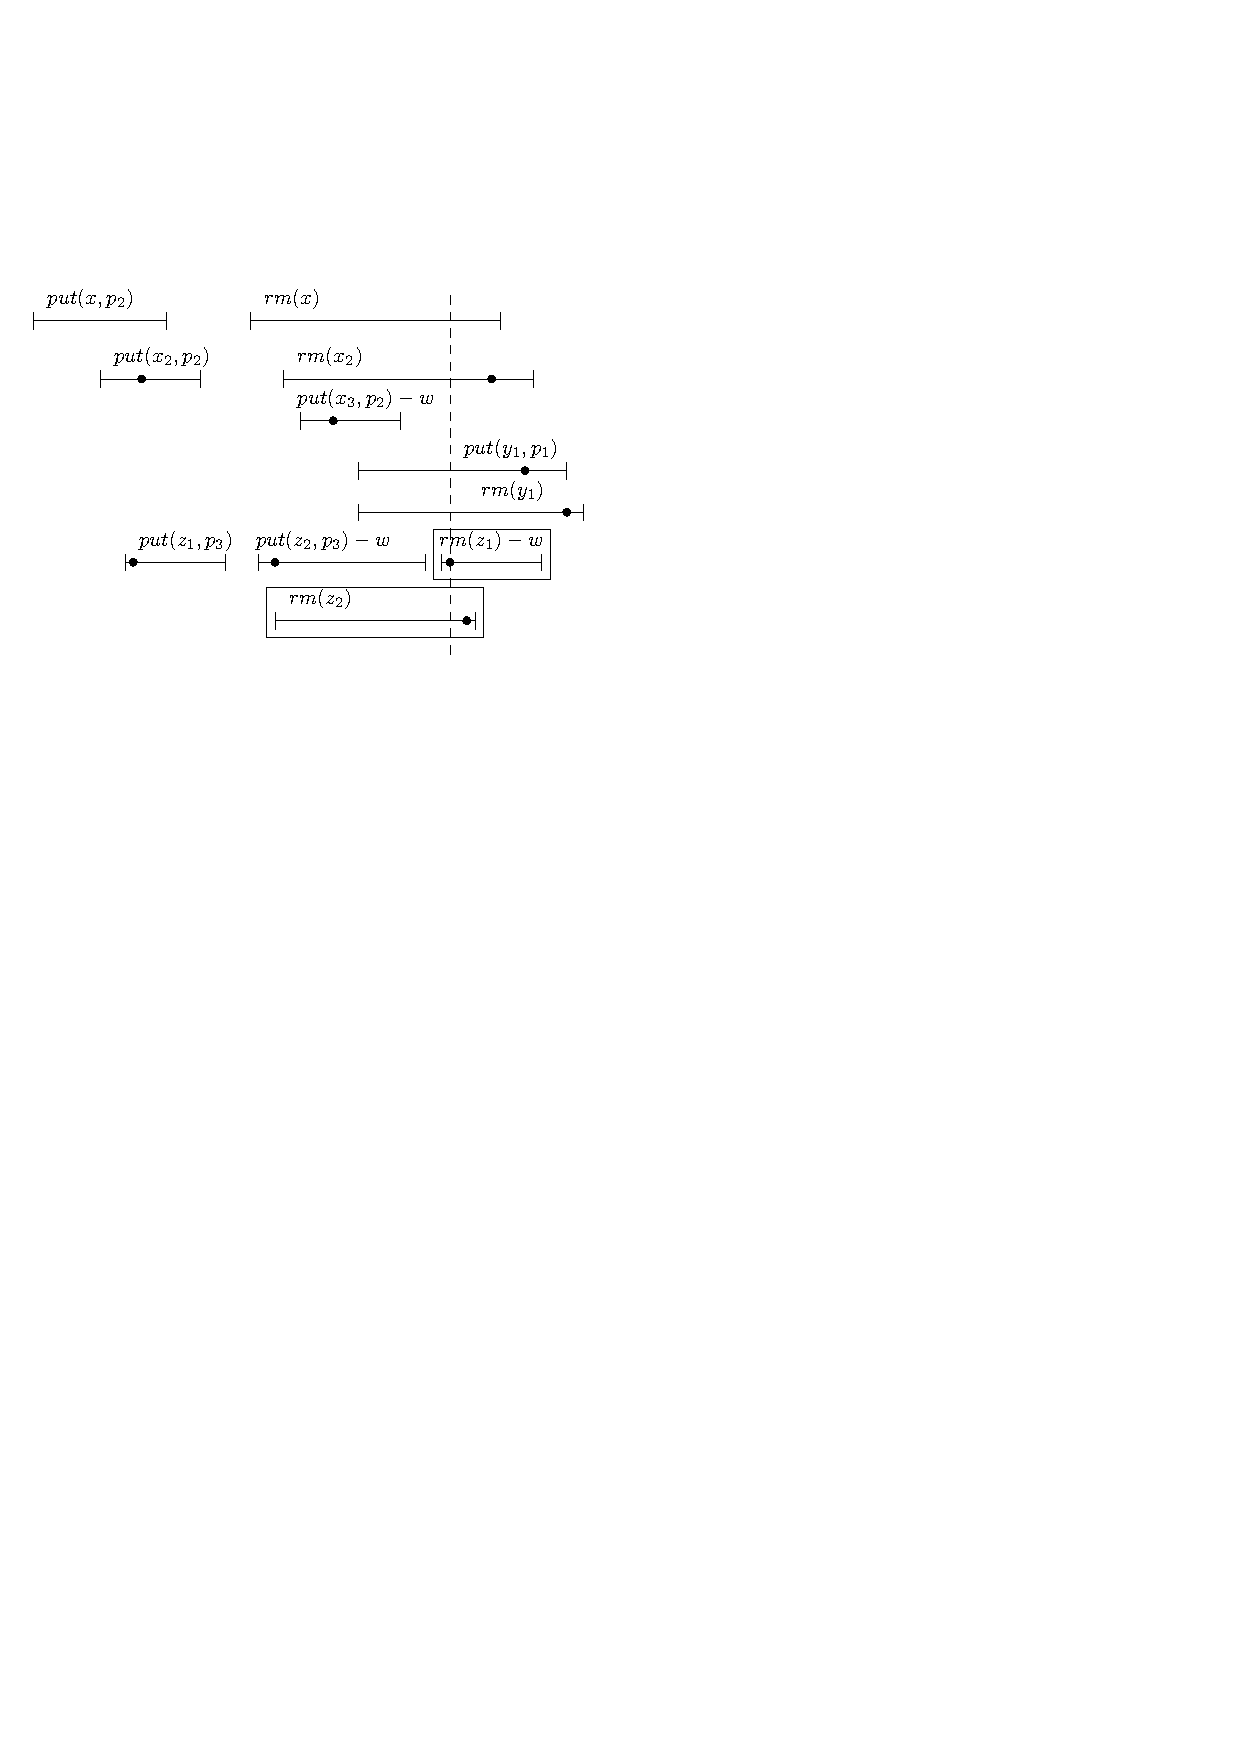
\includegraphics[width=0.5 \textwidth]{figures/PIC-HIS-EPQ1.pdf}
%\vspace{-10pt}
  \caption{Concurrent execution $e$}
  \label{fig:concurrent execution for EPQ1}
\end{figure}


\begin{figure}[htbp]
  \centering
  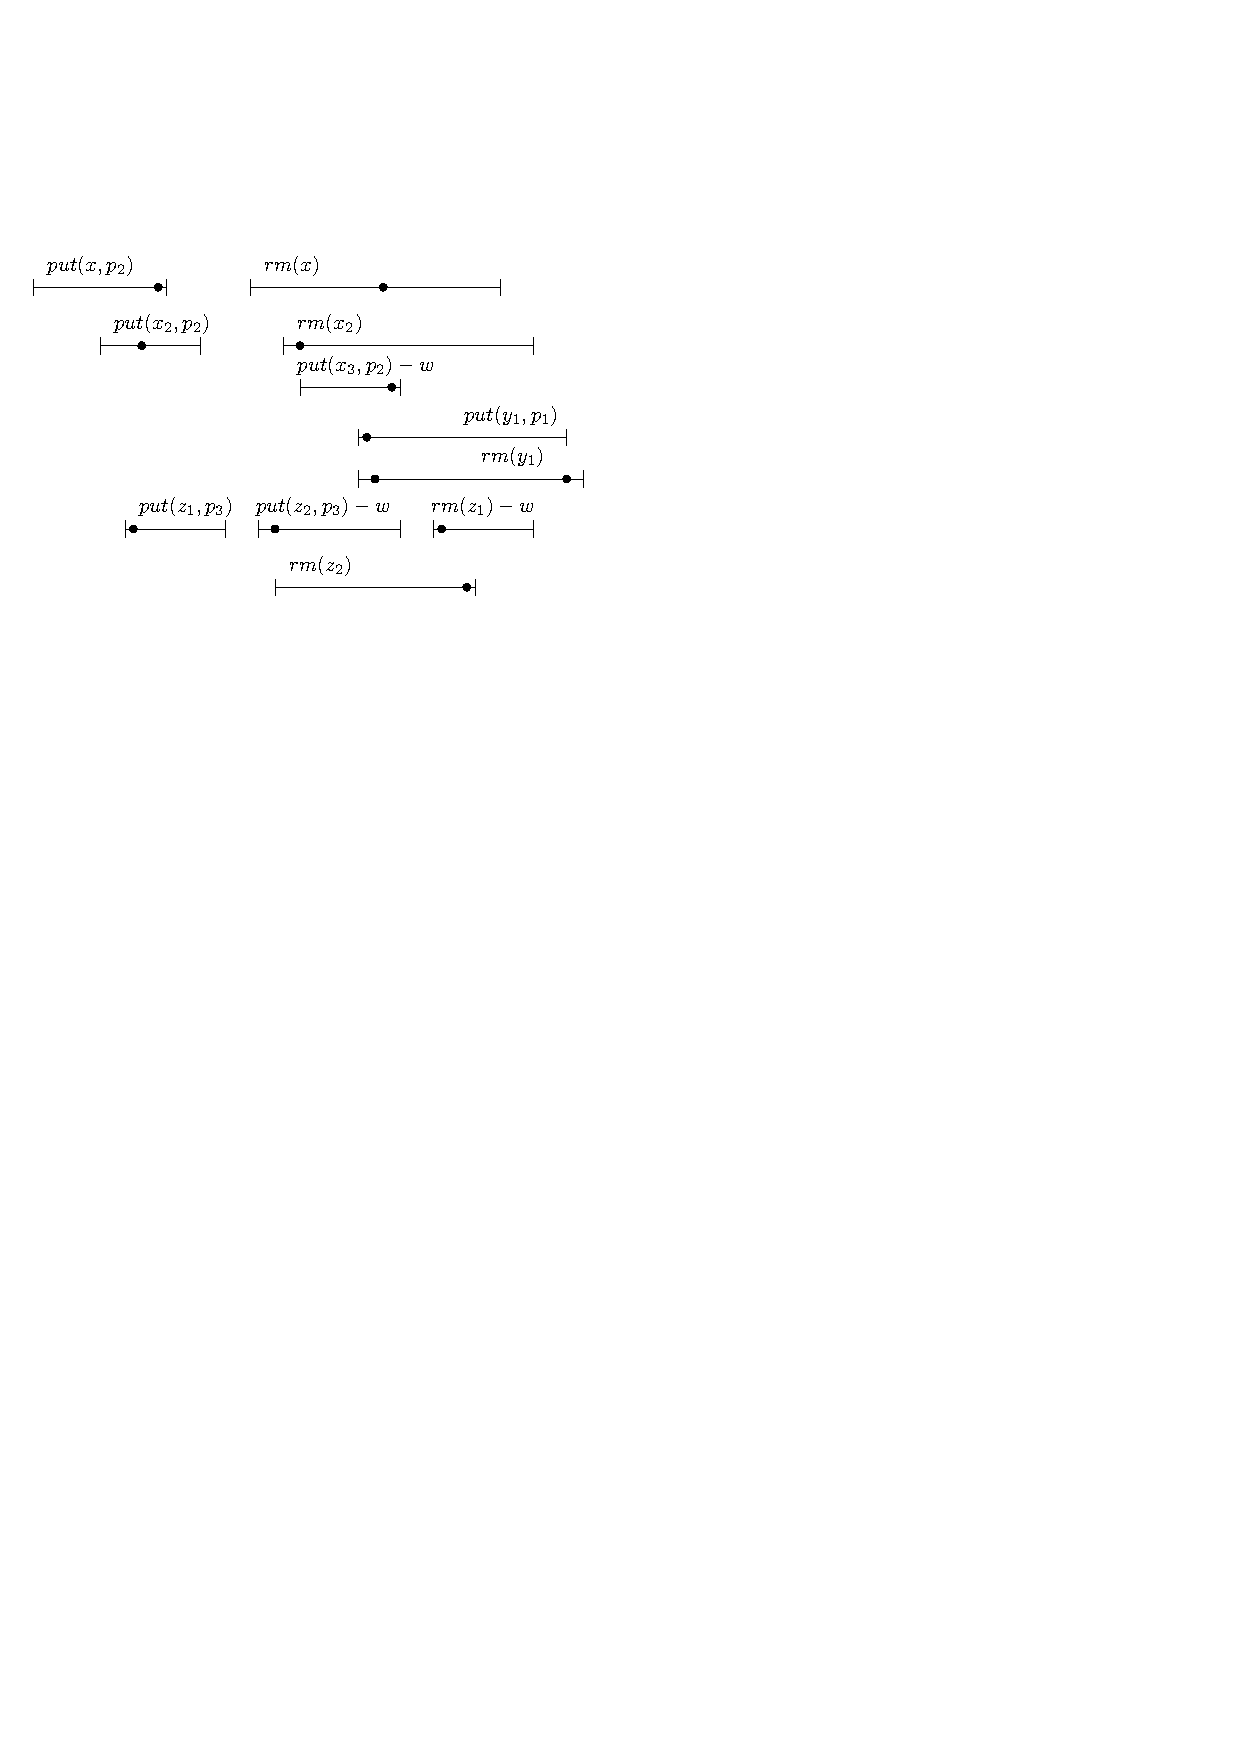
\includegraphics[width=0.5 \textwidth]{figures/PIC-HIS-EPQ1-NEWLP.pdf}
%\vspace{-10pt}
  \caption{Concurrent execution $e$ with linearization points according to $l''$}
  \label{fig:concurrent execution with new linearization points for EPQ1}
\end{figure}


The following lemma states that for data-differentiated execution, checking linearizability with respect to $\textit{EPQ}$ is equivalent to checking linearizability with respect to $\textit{MS}(R)$ for everyone of its projections. Roughly speaking, step-by-step linearizability of extended priority queue play a important rule for proof of the $\textit{if}$ direction of Lemma \ref{lemma:EPQ as multi in MRpri for history}: It guide us how to build a linearization of a whole execution by increasingly construct linearization of sub-execution from $\epsilon$ execution.

\begin{restatable}{lemma}{EPQasMultiInMRpriforHistory}
\label{lemma:EPQ as multi in MRpri for history}
Given a data-differentiated execution $e$, $e \sqsubseteq \textit{EPQ}$, if and only if, $\forall e' \in \textit{proj}(e)$ and $\forall R \in \textit{last}(e')$, we have $e' \sqsubseteq \textit{MS}(R)$.
\end{restatable}
